\chapter{Analysis}

\section{Introduction}

\subsection{Client Identification}

My client is Linh Tham, the owner of Linh's Restaurant. Linh's Restaurant is a family run Chinese restaurant that is situated in small village called Fordham in Cambridgeshire.
 Linh works 'outside' usually on her own where she carries out many roles such as taking phone calls for orders/bookings, serving customers and calculating the bills. Outside is referred as the place where the the serving takes place. When times are busy, relatives come and help out at Linh's Restaurant.

Linh would like a more computerized system to be more efficient as manually transferring order details to the invoice book  can be time consuming. In addition, when it is busy, using time
more efficiently is definitely going to give a better service to the customers and would make it less stressful for Linh. Linh has basic knowledge on how to use a computer such as surfing the internet, checking emails and streaming videos.

\subsection{Define the current system}

Customers come in and get seated according to the number of people. Menus are given and the customers are asked what they would like to drink and what dishes they would like if they are ready. The dishes and drinks are recorded on seperate papers. The top copy of the ordering pad, where the dish order is recorded, is given to the chefs where they cook the dishes and one 
is kept for outside.  Once the dishes are served, the customers are checked upon to see if there are any problems occasionally, and once the customers are satisfied and finish with their meal, they ask for the bill. The recorded order is then copied on to an invoice where the price is calculated for their meal. One invoice is kept
and one is given to the customers. The meal is then paid and the customers leave.

The current system is  paper based. A diary is used for bookings in which customers can book a table over the phone. A name, number of people on the table, a date and time are recorded in the diary.  Orders are taken upfront which is recorded on an ordering pad where one copy is handed over to the kitchen and one is kept to refer to and to transfer order details onto an invoice form.

\subsection{Describe the problems}

When times are busy there could be confusion between on what has been ordered by what table. Also, having to rewrite the order into the invoice book takes time, this is a problem. Furthermore, any inexperienced workers will have to keep referring to the menu when taking orders or calculating the total bill to check if the dish is on the menu and the prices for each dish. This can also lead to a problem where the total price calculated is wrong. Additionally, recorded orders can go missing but that would only happen if the recorded order drops on the floor and no one realises it, this is something that is very unlikely to happen. 


\subsection{Section appendix}

\textbf{Interview with Linh Tham}

\textbf{What is the current system?}

LT : I ask the customers what they would like to eat and drink and record it on an ordering  pad, I then take top copy to the kitchen and keep the second copy for myself so I can refer to who ordered what. Once the customers has finished eating and ready to pay, I transfer all the details from the ordering pad on to the invoice form such as the drinks and dishes with the prices of each. I give a copy of the invoice to the customer and keep one for myself.

\textbf{How are the second copies of the order and invoice created?}

LT : Because of how thin the paper is on the ordering pad ,  writing things down marks down what I write on the second copy. However, the second copies are hard to read because the ink from the pen isn't exactly transferred.

\textbf{What are the problems with the current way of doing things?}

LT : Doing it manually is very time consuming as it takes one person just to rewrite everything on the invoice book. If that one person would be able to finish quicker, that person could help out which would benefit us. 

\textbf{What data or information is recorded in the current system?}

LT : Food items, drinks,total price and the date of an order.

\textbf{What are the benefits of the current system?}

LT : As the system is paper based, any power cuts or weather issues, will not affect how we run the restaurant.

\textbf{What should the new system be able to do?}

LT : Having a way to look at what tables have ordered what, like a simulator, this will help the restaurant staff to keep track of tables and will reduce confusion. Storing sit down orders would be helpful also.

Having a way to look at what tables have ordered what, like a simulator, this will help the restaurant staff to keep track of tables and will reduce confusion. Storing sit down orders would be helpful also.

\textbf{Would you like to store phone call orders?}

LT: No, I would only like to store sit down orders.

\textbf{How long would you like to store the information?}

LT: I would like to store the information for 3 months.


\section{Investigation}

\subsection{The current system}

\subsubsection{Data sources and destinations}

There are two main data sources in the current system, the menu and the customer. The menu contains foods and drinks the customer can choose from, the restaurant staff takes the order and  then writes down the drinks and dishes onto seperate ordering pads without prices. The details of the order is copied onto the invoice including prices and the date once the customer is finished. Each dish ordered is recorded on the invoice however, each drink ordered isnt and so the total price of drinks ordered is recorded instead and referred as 'Drinks' on the invoice form. Additionally, the number of people on the table isn't recorded on the invoice.
\begin{center}

\begin{tabular}{ | p{2cm} | p{3cm} | p{3cm} | p{2cm} |  }
    \hline
    \textbf{Source} & \textbf{Data} & \textbf{Example Data} & \textbf{Destination} \\ \hline
    Menu & Drink and dishes with prices &Orange Juice £0.70 \newline Special fried rice £3.70 & Customer \\ \hline
    Customer & Drink &Bottled water &Restaurant staff \\ \hline
    Customer & Dish &Wonton soup&Restaurant staff \\ \hline
   Restaurant staff &Drink ordered by customer, table number &Bottled water\newline Sprite \newline Table No. 3 & Ordering pad 1 \\ \hline
   Restaurant staff &Dish ordered by customer, date of order, number of people, table number&Wonton soup \newline Special fried rice \newline 30/9/14 \newline Covers 2 \newline Table No. 3& Ordering pad 2 \\ \hline
   Ordering pad 1 &Total price of drinks - each drink is not specified on invoice, \newline table number &(£0.60+£0.70) \newline Total £1.30 \newline Table No. 3 & Invoice pad \\ \hline
   Ordering pad 2 &Dishes ordered by customer including price of each dish, \newline table number & Wonton soup £1.80 \newline Special fried rice £3.70 \newline Table No. 3  & Invoice pad \\ \hline
   Restaurant staff & Total price of order & Total price £6.8 & Invoice pad \\ \hline
   Invoice pad& Copy of invoice & Wonton soup £1.70 \newline Special fried rice £3.70 \newline  Drinks £1.30 \newline Total price £6.8\newline  Date 30/9/14   \newline Table No. 3& Customer \\ \hline

    \hline
\end{tabular}
\label{tab:range_examples}
\end{center}

\newpage

\subsubsection{Algorithms}

\begin{algorithm}[H]
\label{fig:Order_from_customer}
    \caption{Taking an order}
\begin{algorithmic}[1]
\SET{$OrderTaken$}{$false$}
\State
\While{$not OrderTaken$}
    \If{Customer ready to order}
    \RECEIVE{$Order$}
    \SET{$OrderTaken$}{$true$}
    \Else \\
     \indent{Wait}
    \EndIf
\EndWhile
\end{algorithmic}
\end{algorithm}

\begin{algorithm}[H]
\label{fig:Generate_invoice}
    \caption{Generating invoice}
\begin{algorithmic}[1]
\SET{$InvoiceGenerated$}{$false$}
\State
\While{$not InvoiceGenerated$}
    \If{Customer has finished ordering} \\
Copy order details from order pad onto invoice pad \\ 
Get prices of each dish and drink ordered from menu \\
Copy prices onto invoice pad \\
Calculate total price \\
Add date 
    \SET{$InvoiceGenerated$}{$true$}
    \Else \\
     \indent{Wait for customer to ask for the bill}
    \EndIf
\EndWhile
\end{algorithmic}
\end{algorithm}

\begin{algorithm}[H]
\label{fig:Payment_from_customer}
    \caption{Payment}
\begin{algorithmic}[1]
\SET{$Payment$}{$false$}
\State
\While{$not Payment$}
    \If{Customer ask for bill} \\
	Give invoice
    \RECEIVE{$Payment$}
    \SET{$Payment$}{$true$}
    \Else \\
     \indent{Wait}
    \EndIf
\EndWhile
\end{algorithmic}
\end{algorithm}

\newpage

\subsubsection{Data flow diagram}

\begin{figure}[H]
    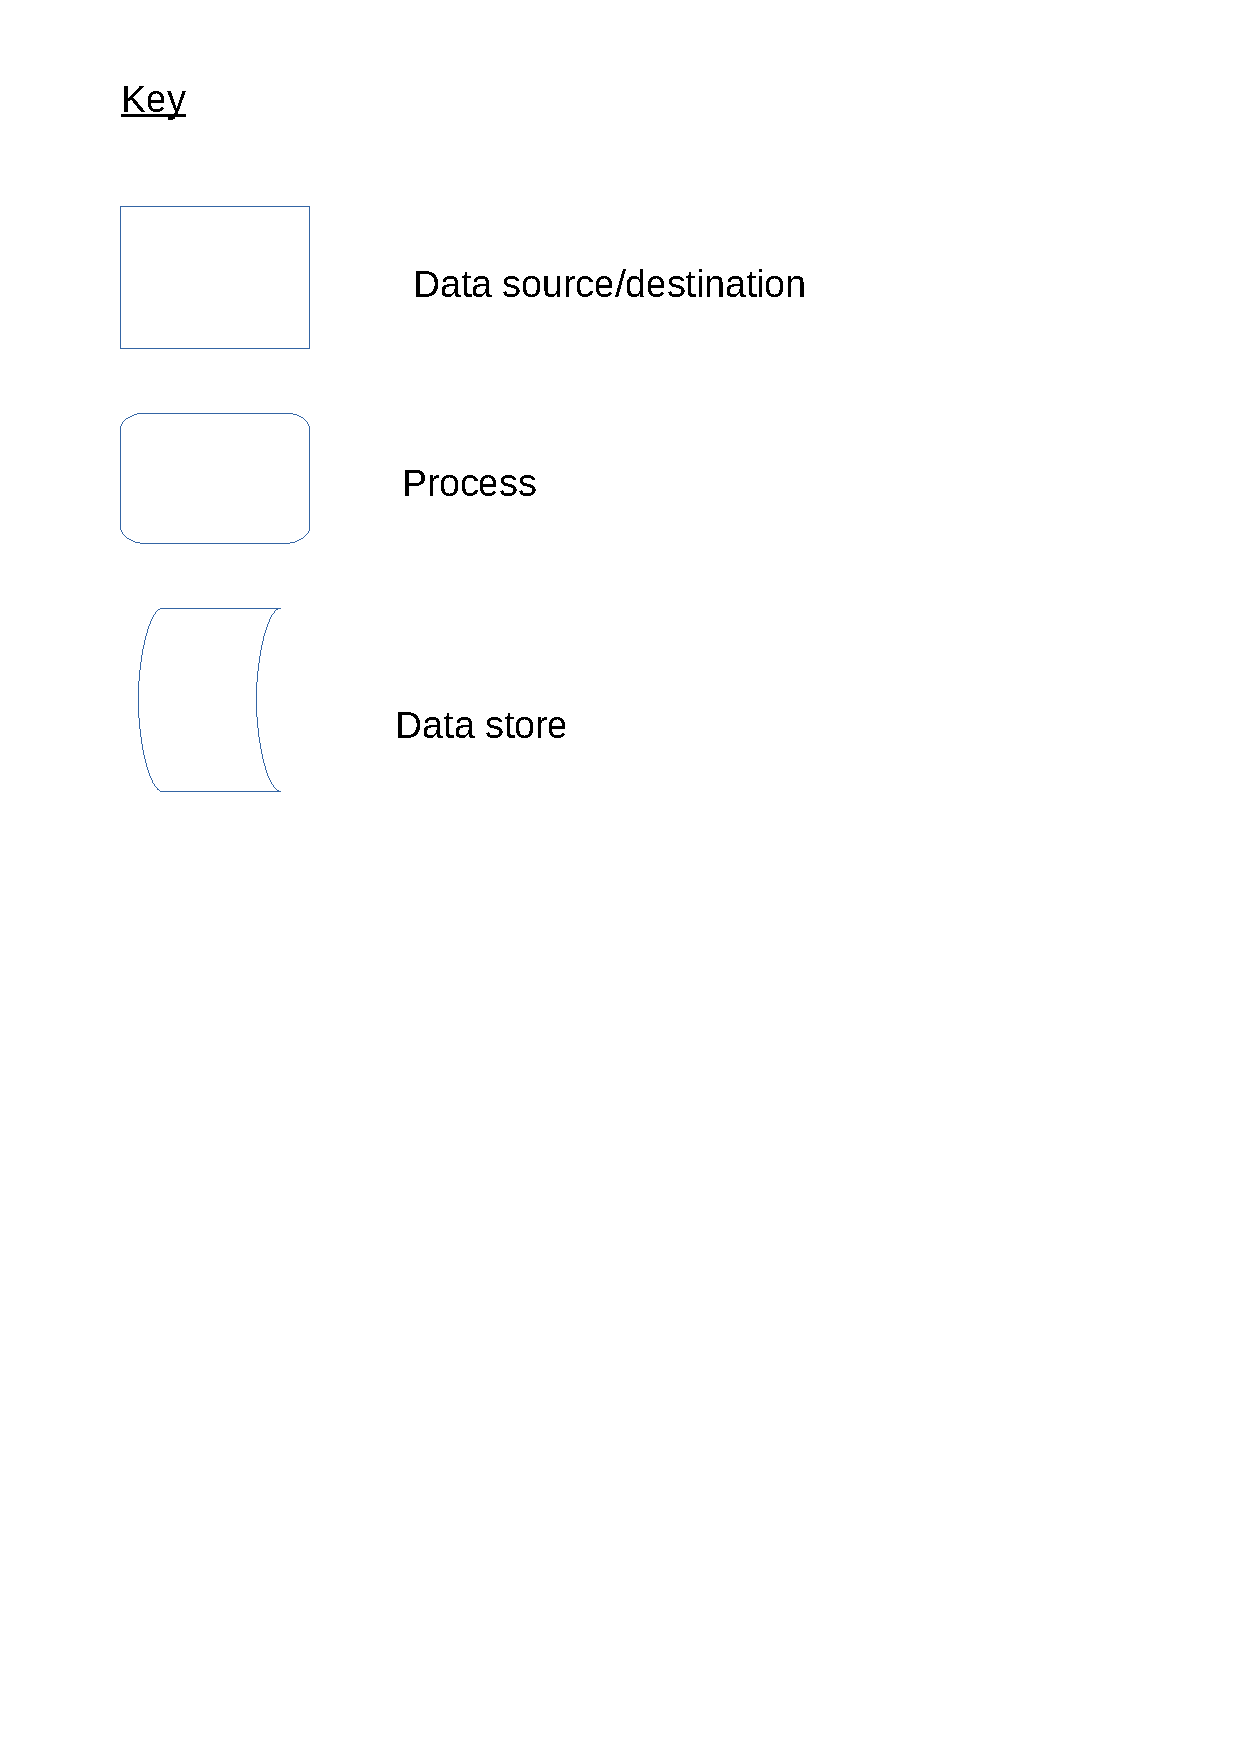
\includegraphics[height = 18cm]{./Analysis/Dataflowkey}
    \caption{Data flow key} \label{fig:flow_key}
\end{figure}

\begin{figure}[H]
    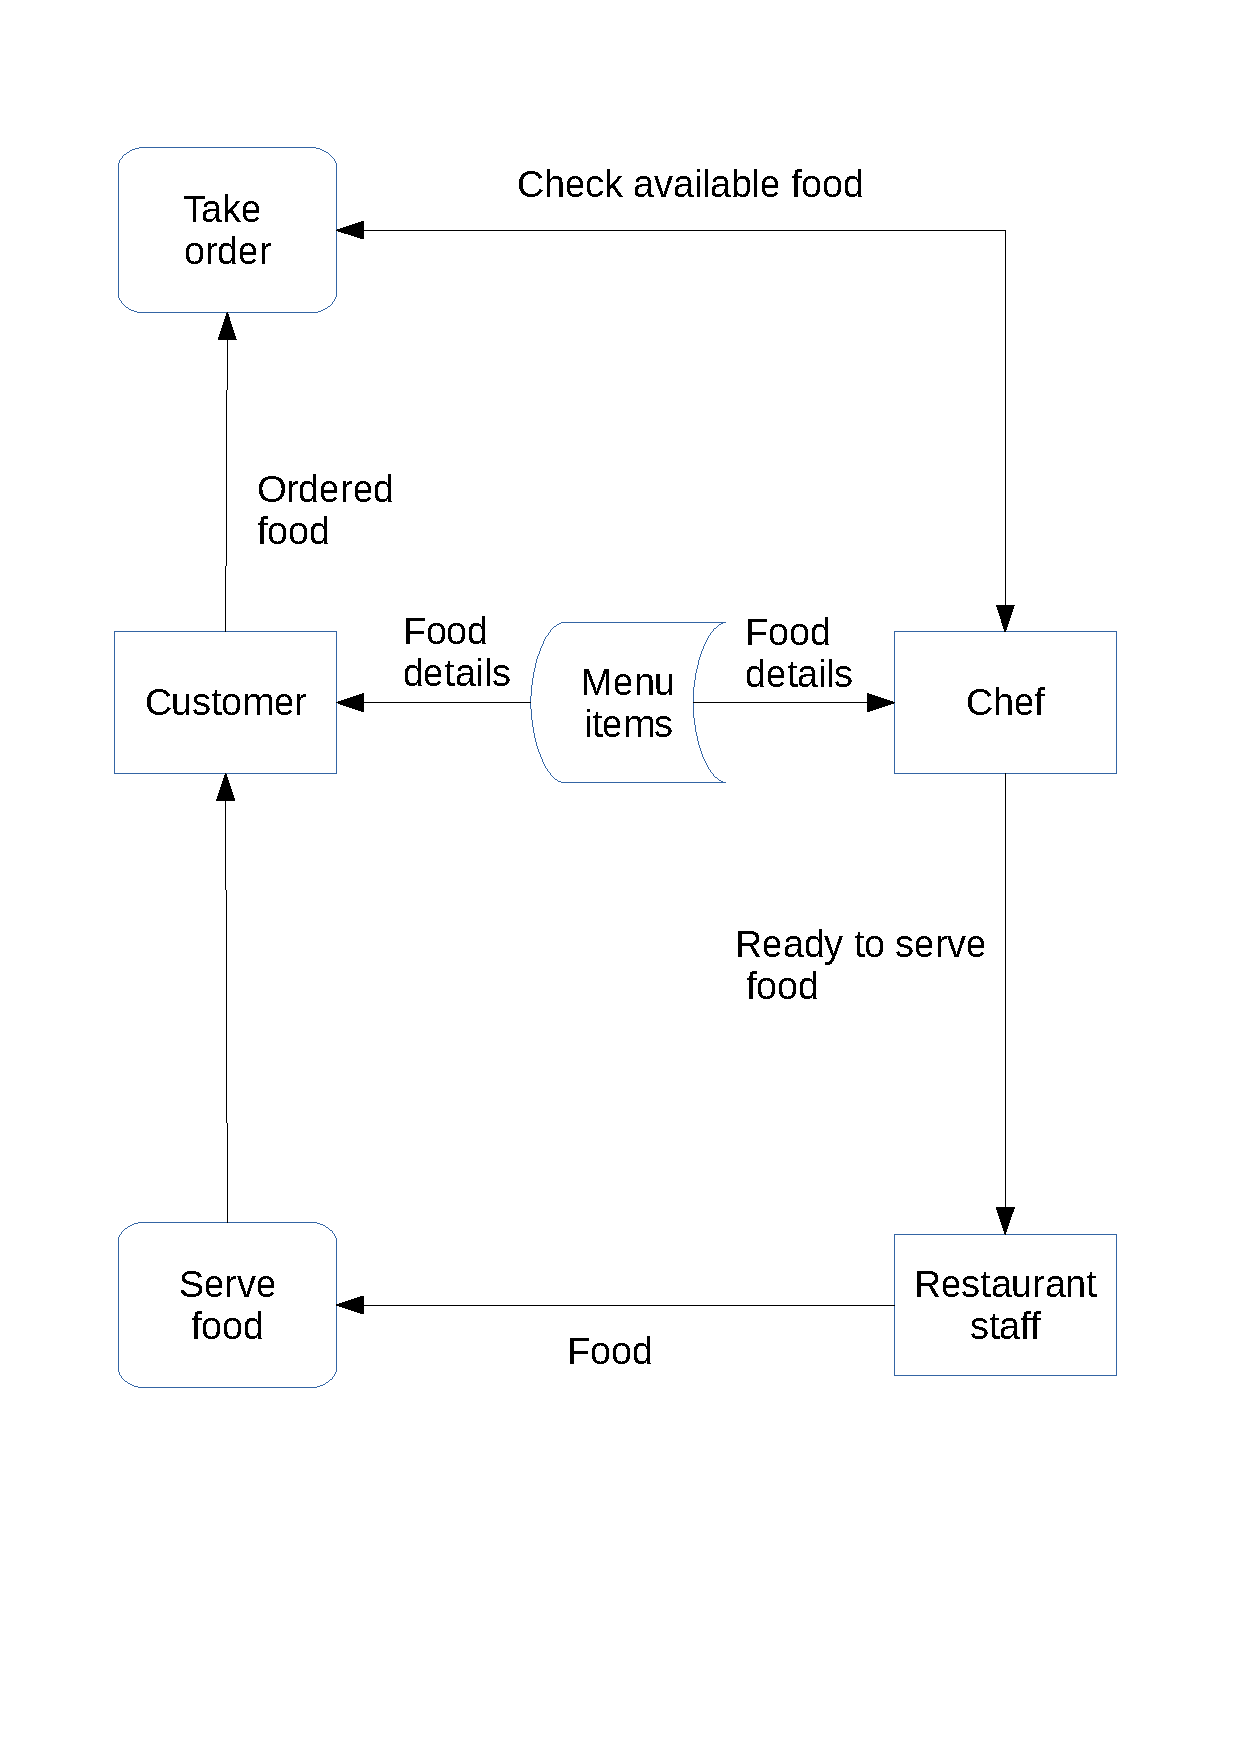
\includegraphics[height = 18cm]{./Analysis/PlacingOrder}
    \caption{Data flow diagram of placing an order} \label{fig:Data_flow_diagram}
\end{figure}

\begin{figure}[H]
    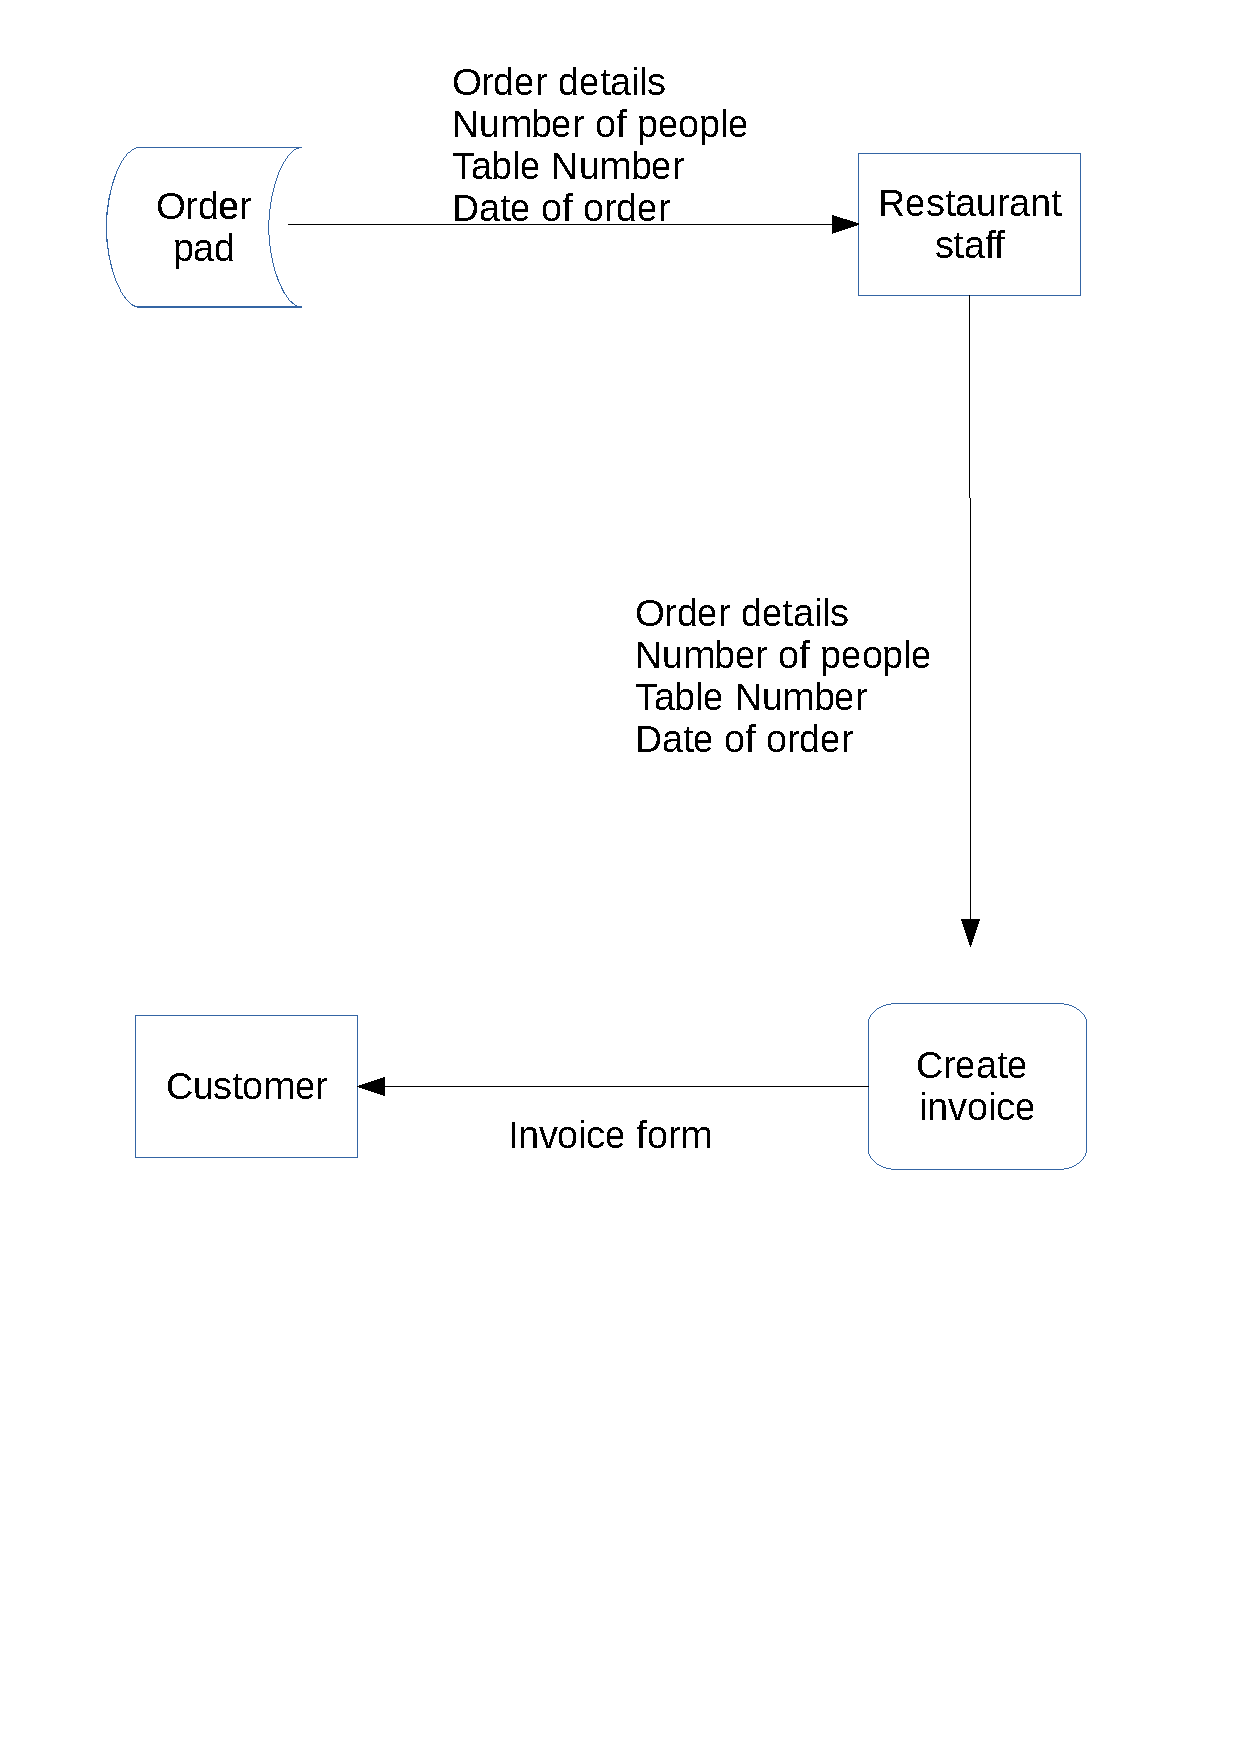
\includegraphics[height = 18cm]{./Analysis/InvoiceGeneration}
    \caption{Data flow diagram of generating an invoice} \label{fig:Data_flow_diagram}
\end{figure}

\subsubsection{Input Forms, Output Forms, Report Formats}
Drinks are recorded seperately from dishes as shown below. The number at the top represents what table number this order is from.


\begin{figure}[H]
    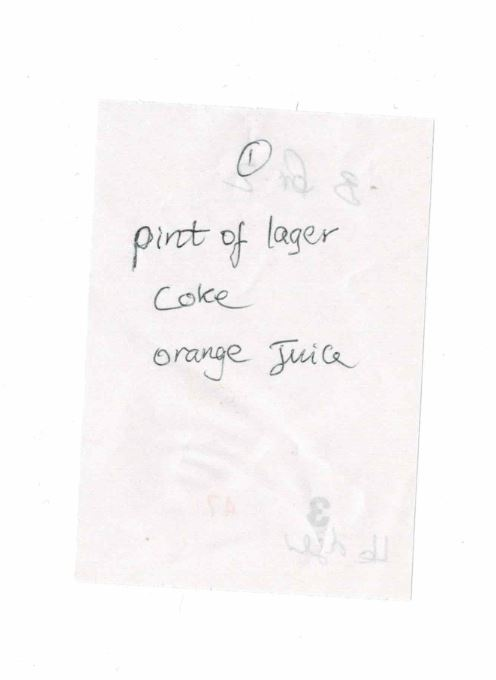
\includegraphics[height = 12cm]{./Analysis/DrinkPad}
    \caption{Writing down drinks ordered on the drink pad} \label{fig:order_pad}
\end{figure}
\newpage

Below is an example of what the ordering pad looks like when a customer's order has been taken. It provides information about the order such as the table number, how many people is seated, dishes ordered and the date the order has taken place. Two copies of this is made, one is taken to the chefs and one is kept for the waitors. This is an input form.


\begin{figure}[H]
    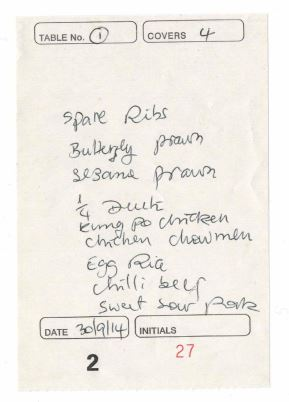
\includegraphics[height = 12cm]{./Analysis/DishPad}
    \caption{Getting an order from a customer} \label{fig:order_pad}
\end{figure}


\newpage
A picture of an invoice is shown below, the information has been transferred from the ordering pad, as shown above, to the invoice pad. An invoice is created once a table has finished eating and ready to pay. Only the date, description, prices and total price is put on the invoice. This is an output which is given to the customers and another copy of the invoice is kept.

\begin{figure}[H]
    \includegraphics[height = 14cm]{./Analysis/Invoice}
    \caption{Creating invoice} \label{fig:invoice}
\end{figure}

\subsection{The proposed system}

\subsubsection{Data sources and destinations}

In the proposed system, getting an order from the customer is still the same via using restaurant staff and an order pad. The only change in the propose system is transferring the order details onto an invoice. 

\begin{center}

\begin{tabular}{ | p{2cm}| p{3cm} | p{2cm} | p{2cm} |  }
    \hline
    \textbf{Source} & \textbf{Data} & \textbf{Example Data} & \textbf{Destination} \\ \hline
    Menu &Dish and drink & Spare ribs, orange juice &Customer \\ \hline
    Customer &Drink ordered & Orange juice &Restaurant staff \\ \hline
    Customer & Dish ordered & Wonton soup& Restaurant staff \\ \hline
    Restaurant staff &Drink ordered by customer, \newline table number & Orange juice  \newline Table No. 1& Ordering pad \\ \hline
    Restaurant staff & Dish ordered by customer, \newline table number, number of people, \newline date of order & Wonton soup, \newline Table No. 1, \newline Covers 1 \newline 04/09/14 & Ordering pad \\ \hline
    Proposed system software & Invoice form & 04/09/14 \newline Wontop soup £ 1.80 \newline Drinks £0.7 \newline Total price £2.50 & Customer  \\ 
    \hline
\end{tabular}
\label{tab:range_examples}
\end{center}

\newpage

\begin{center}

The new part of the system's data sources and destinations is shown below. Entering the food item onto the software should automatically retrieve its price from the menu database. After a customer has finished with their meal, the simulator saves the Table status ( drinks, dishes, table number and date) to the order history database and creates an invoice form.

\begin{tabular}{ | p{3cm} | p{3cm} | p{1cm} | p{3cm} |  }
    \hline
    \textbf{Source} & \textbf{Data} & \textbf{Data type} & \textbf{Destination} \\ \hline
    Restaurant staff &Dish & String &Computer - Table status \\ \hline
   Restaurant staff & Drink & String & Computer - Table status \\ \hline
  Restaurant staff & TableNumber &Integer & Computer - Table status \\ \hline
    Restaurant staff & NumberOfPeople &Integer &Computer - Table status \\ \hline
    Restaurant staff & DateOfOrder & Date & Computer - Table status \\ \hline
   Computer - Table status & OrderID  & Integer & Database - Order records  \\ \hline
   Computer - Table status & Dish  & String & Database - Order records  \\ \hline
   Computer - Table status & Drink  & String & Database - Order records  \\ \hline
   Computer - Table status & TableNumber  & Integer & Database - Order records  \\ \hline
   Computer - Table status & DateOfOrder  & Date & Database - Order records  \\ \hline
   Computer - Table status & TotalDrinkPrice & Float & Database - Order records  \\ \hline
   Computer - Table status & TotalPrice \newline (TotalDrinkPrice + each dish) & Float &Database - Order records  \\ \hline
   Computer - Table status & InvoiceForm & string & InvoiceFolder  \\ \hline

\end{tabular}
\label{tab:range_examples}
\end{center}

\newpage

\subsubsection{Data flow diagram}

The data flow diagram of placing an order will be the same due to no changes to the way of placing and processing the order.

\begin{figure}[H]
    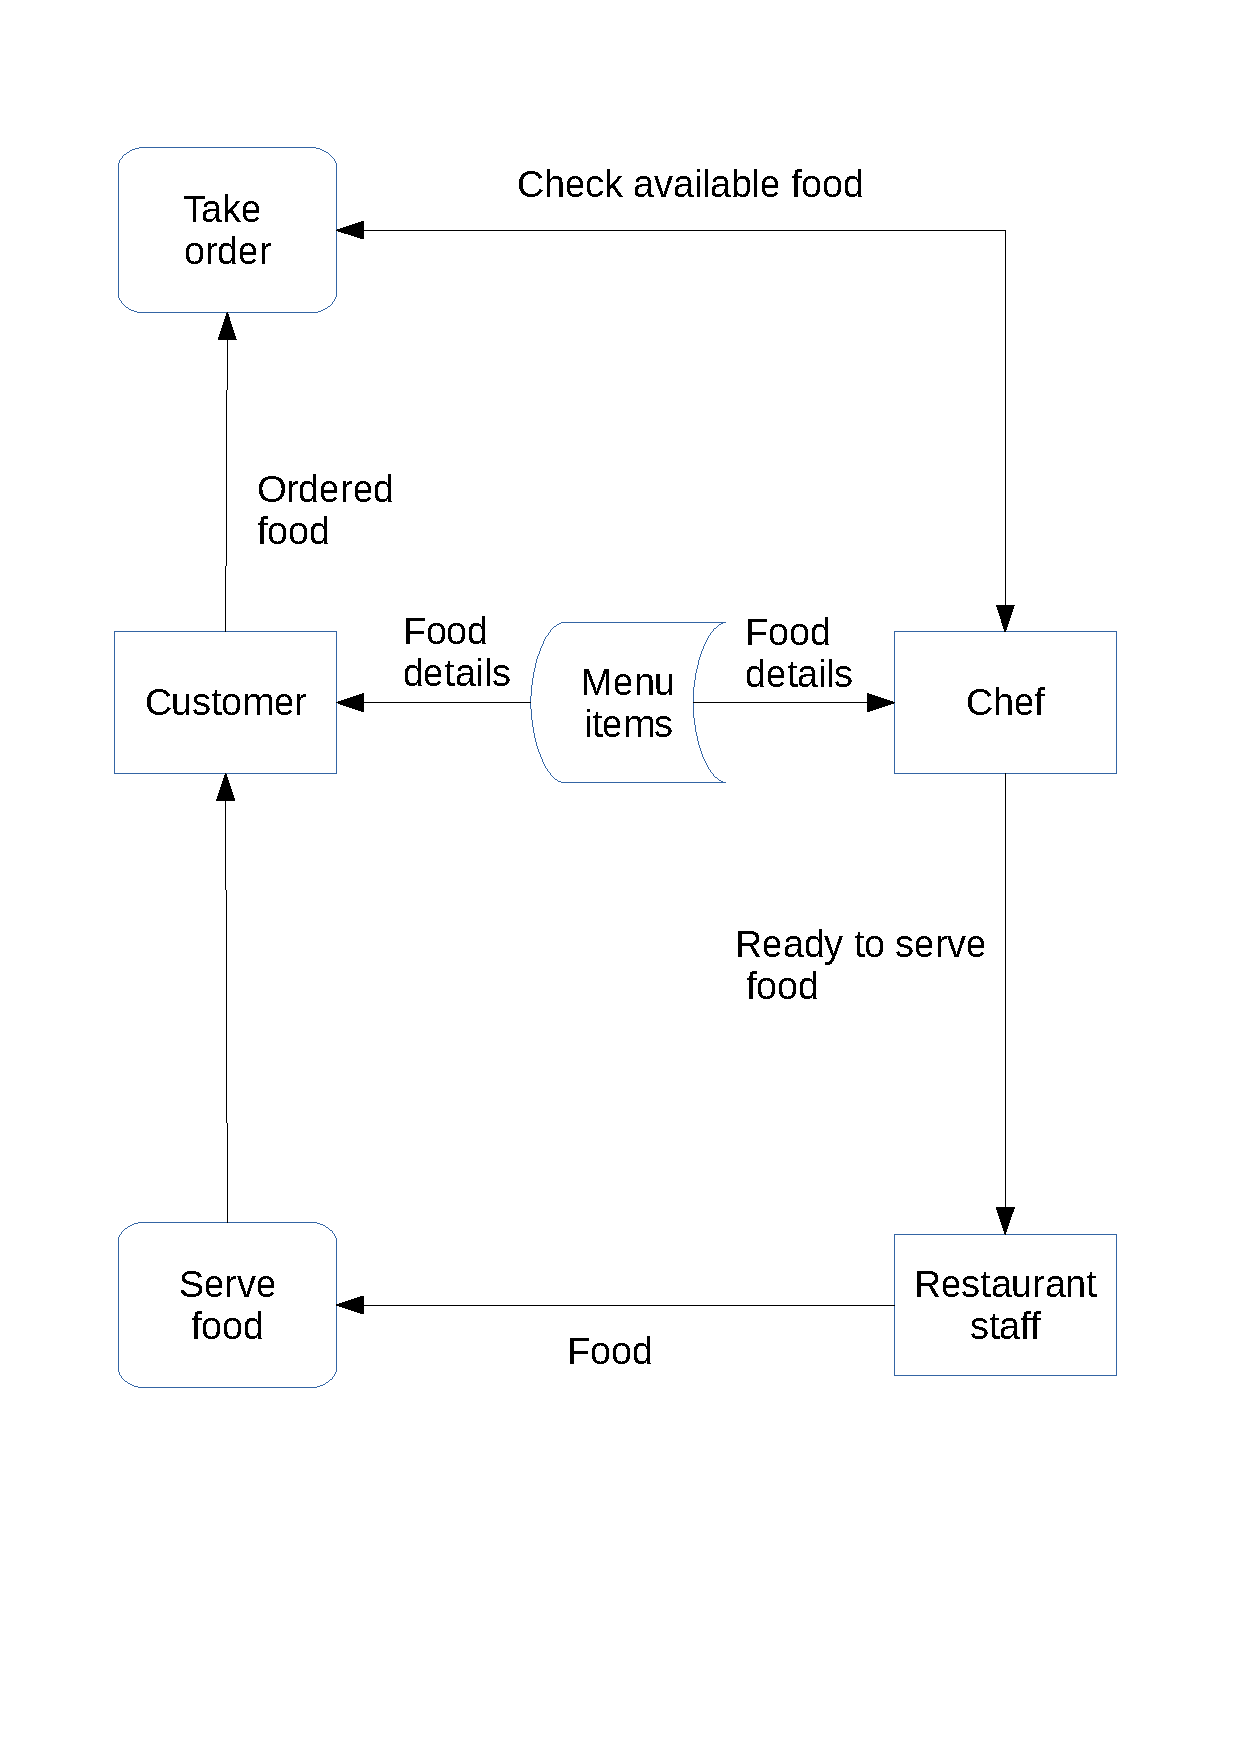
\includegraphics[height = 16cm]{./Analysis/PlacingOrder}
    \caption{A data flow diagram of the proposed system - placing and processing the order} \label{fig:Restaurantflow}
\end{figure}

\newpage

The proposed system will make the restaurant staff input data into the system which will be shown on the application if the user checks what table has ordered what. In addition the inputed data saved in a database once the customer has finished with their meal. Also, invoices will be created though this application.

\begin{figure}[H]
    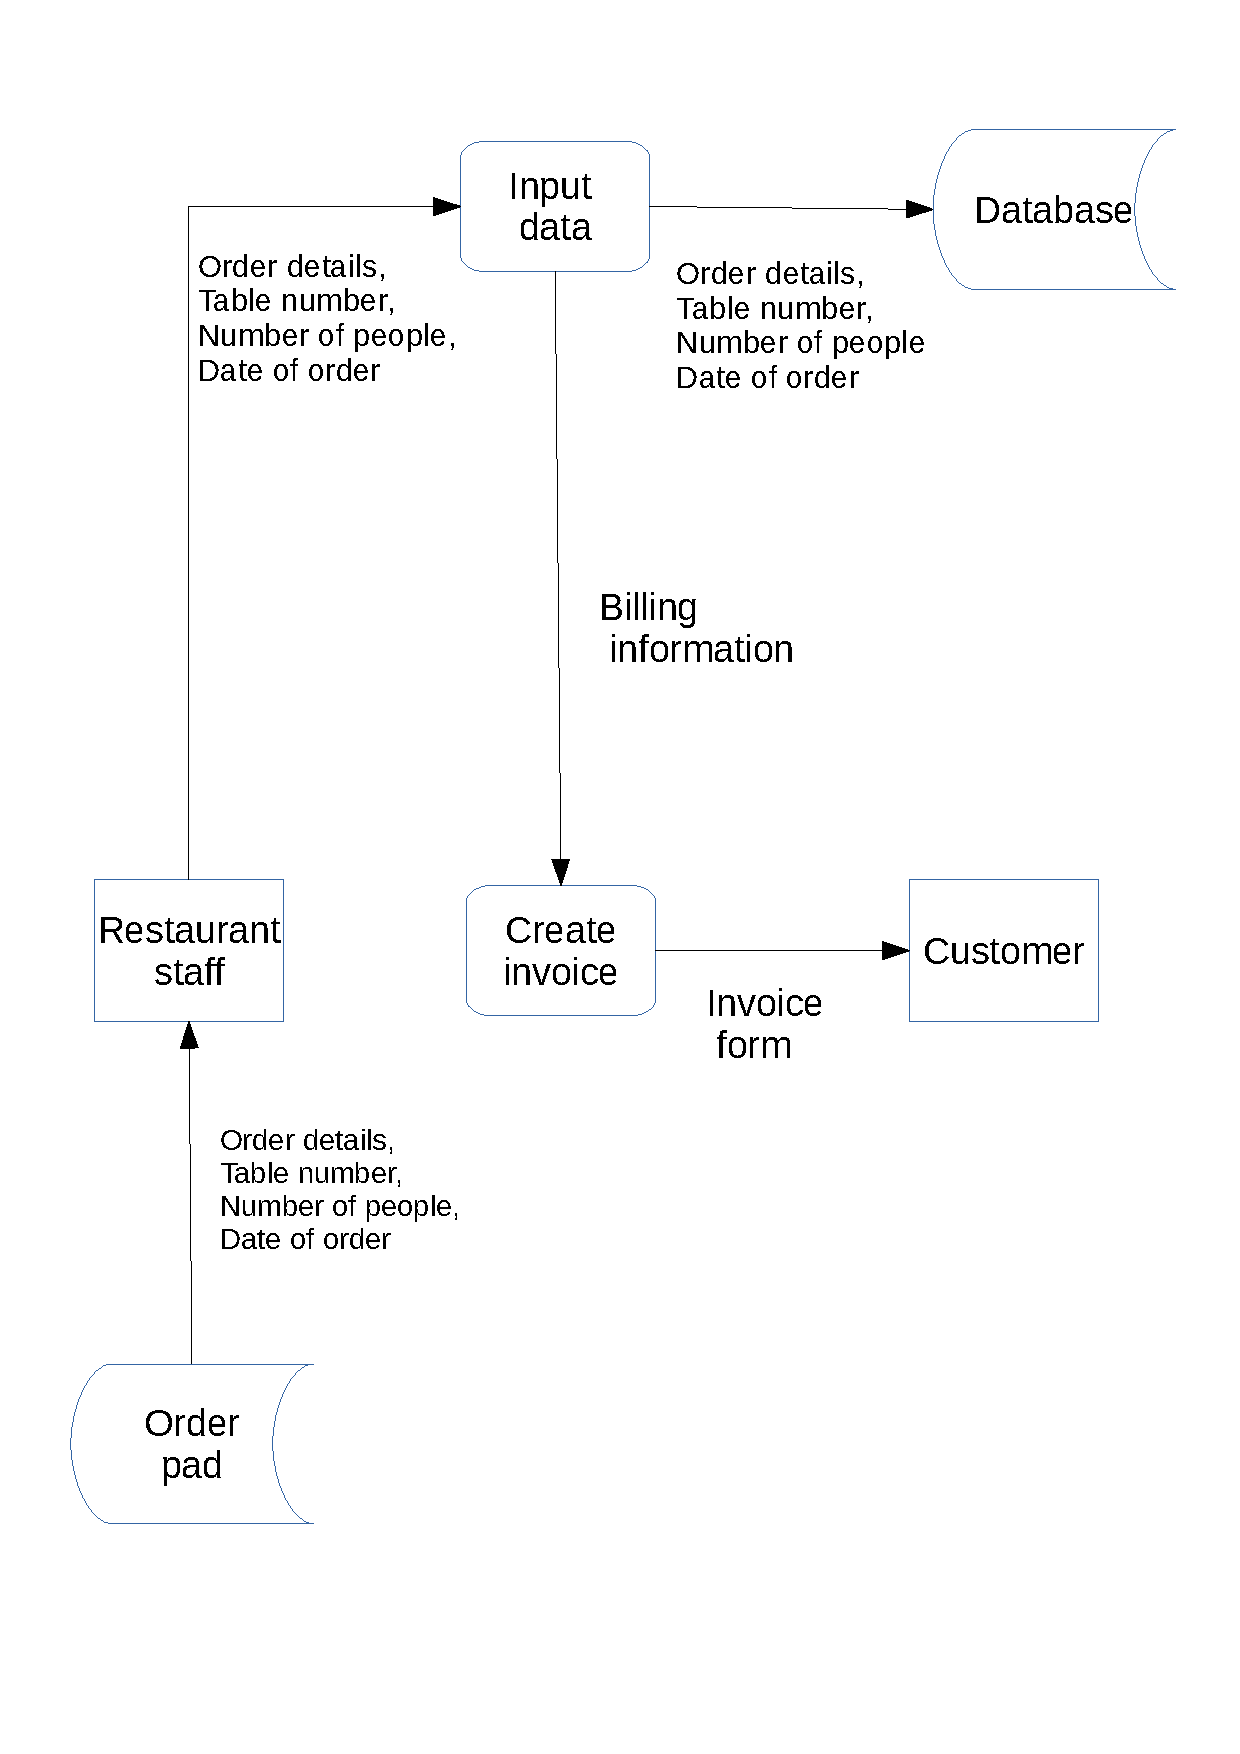
\includegraphics[height = 16cm]{./Analysis/ProposeInvoice}
    \caption{Data flow diagram proposed system} \label{fig:Invoiceflow}
\end{figure}

\subsubsection{Data dictionary}

\begin{center}

\begin{tabular}{ | p{3cm}| p{1cm} | p{2cm} | p{2cm} | p{2cm} |  }
    \hline
    \textbf{Name} & \textbf{Data Type} & \textbf{Length} & \textbf{Validation} &\textbf{Example Data} \\ \hline
   TableNumber & Integer & 1 - 16 & Range  & 13\\ \hline
   NumberOfPeople & Integer & 1 - 20 & Range  & 4 \\ \hline
   MenuItem & String & 1 - 20 Characters & Length  & Spare ribs\\ \hline
   ItemQuantity & Integer & 1 - 10 & Range  & 4\\ \hline
   ItemPrice & Float & 0 - 20 & Range  &3.2\\ \hline
    TotalPrice & Float & 0 - 500 & Range  & 54.4\\ \hline
   DateOfOrder &Date & 4 - 6 & Format  & 16/11/14\\ \hline
    InvoiceCreated & Boolean &  & Presence Check  & \\ \hline


\end{tabular}
\label{tab:range_examples}
\end{center}


\subsubsection{Volumetrics}

As an ascii character is 1 byte, there will be 35 bytes for one sitdown order. 35*30(approximately the max sit down orders per day) = 1050 bytes is stored per day. Linh's restaurant is open 6 days a week so 1050*6 = 6300 bytes and  Linh has stated that she would like to store the information for 3 months so  6300*13.2(weeks) = 83160 bytes will need to be stored.

81360 bytes is equivalent to 79.45 kilobytes (81360/1024). 79.45 kb would be needed to store 3 months of information. The software it self will contain pictures which will increase the size by roughly 2MB. Therefore the total space required would be 6MB if the application itself took 4MB without any images ( 2MB + 4MB).





\section{Objectives}

\subsection{General Objectives}

\begin {itemize}
	\item Create a restaurant simulator  to track orders
	\item Simple and clear GUI for user-friendly experience.
	\item Having the ability to easily modify orders.
	\item Create a digital invoice after table has finished their meal.
	\item Storing orders.
\end {itemize}

\newpage 

\subsection{Specific Objectives}

Simple and clear GUI
\begin {itemize}
	\item Having a very simple birds eye view image of the restaurant which is made out of shapes to ease the understanding of where each table is.
	\item Label table with their corresponding number.
	\item Table shapes will be big so it won't be hard to click on them but not so big that 16 tables can fit on the GUI.
	\item Clicking on table will bring up a window which shows the status such as the date and food items ordered with noticeable order modification options.
\end {itemize} 

Order alterations 
\begin{itemize}
	\item Have clear Add, Delete  and Create invoice buttons.
	\item When user chooses the add option, have an input box appear where user can type in an ID for a dish/drink or the actual name of the dish/drink.
	\item Make the input search function not case sensitive.
	\item When user wants to delete a food item off the list, have clear red X boxes appear next to the name. When red X boxes are clicked on and with confirmation, the item gets deleted.
	\item Have an up arrow or bottom arrow button just in case a customer orders another food item which is already on the list. The up arrow would increase the quantity of the item by 1 and the down arrow would 		decrease the item by 1 .
	\item Clicking on create invoice button will clear the information on the table status and save the digital invoice in a folder.
\end{itemize} 

Track orders
\begin{itemize}
	\item Drinks and dishes will be seperated by columns.
	\item Clicking on a table will bring up a small window with the list of food items that the table has ordered, formatted like the invoice form shown on page 15. This also includes the date and table number.
 
\end{itemize}

Invoice creation 
\begin{itemize}
	\item Automatically creating a digital invoice when a customer has finished.
	\item Calculate total price
	\item The digital invoice will look very similar to the invoice on page 15.
	\item Invoice will contain the items ordered, prices of each and total price.
	\item Have the option to print out invoice.
\end{itemize} 

Storing orders
\begin{itemize}
	\item When using the clear information button, the information is stored in the database.
	\item Filtering database for user if searching specific information.
	\item Have an option to view database.
\end{itemize}

\subsection{Core Objectives}

\begin{itemize}
	\item Have a working simulator that will have the restaurant layout
	\item Having clickable tables that will bring up a window showing a digital invoice
	\item The digital invoice will show the current status such as items ordered, date of order and number of people on the table.
	\item Application must be able to modify orders
	\item Application must be able to generate an invoice after table has finished with their meal
\end{itemize} 

\subsection{Other Objectives}


\begin{itemize}
	\item Print invoice function
	\item Store order data in a database
	\item Database search functions such as sort and filtering.
\end{itemize} 

\section{ER Diagrams and Descriptions}

\subsection{ER Diagram}

\begin{figure}[H]
    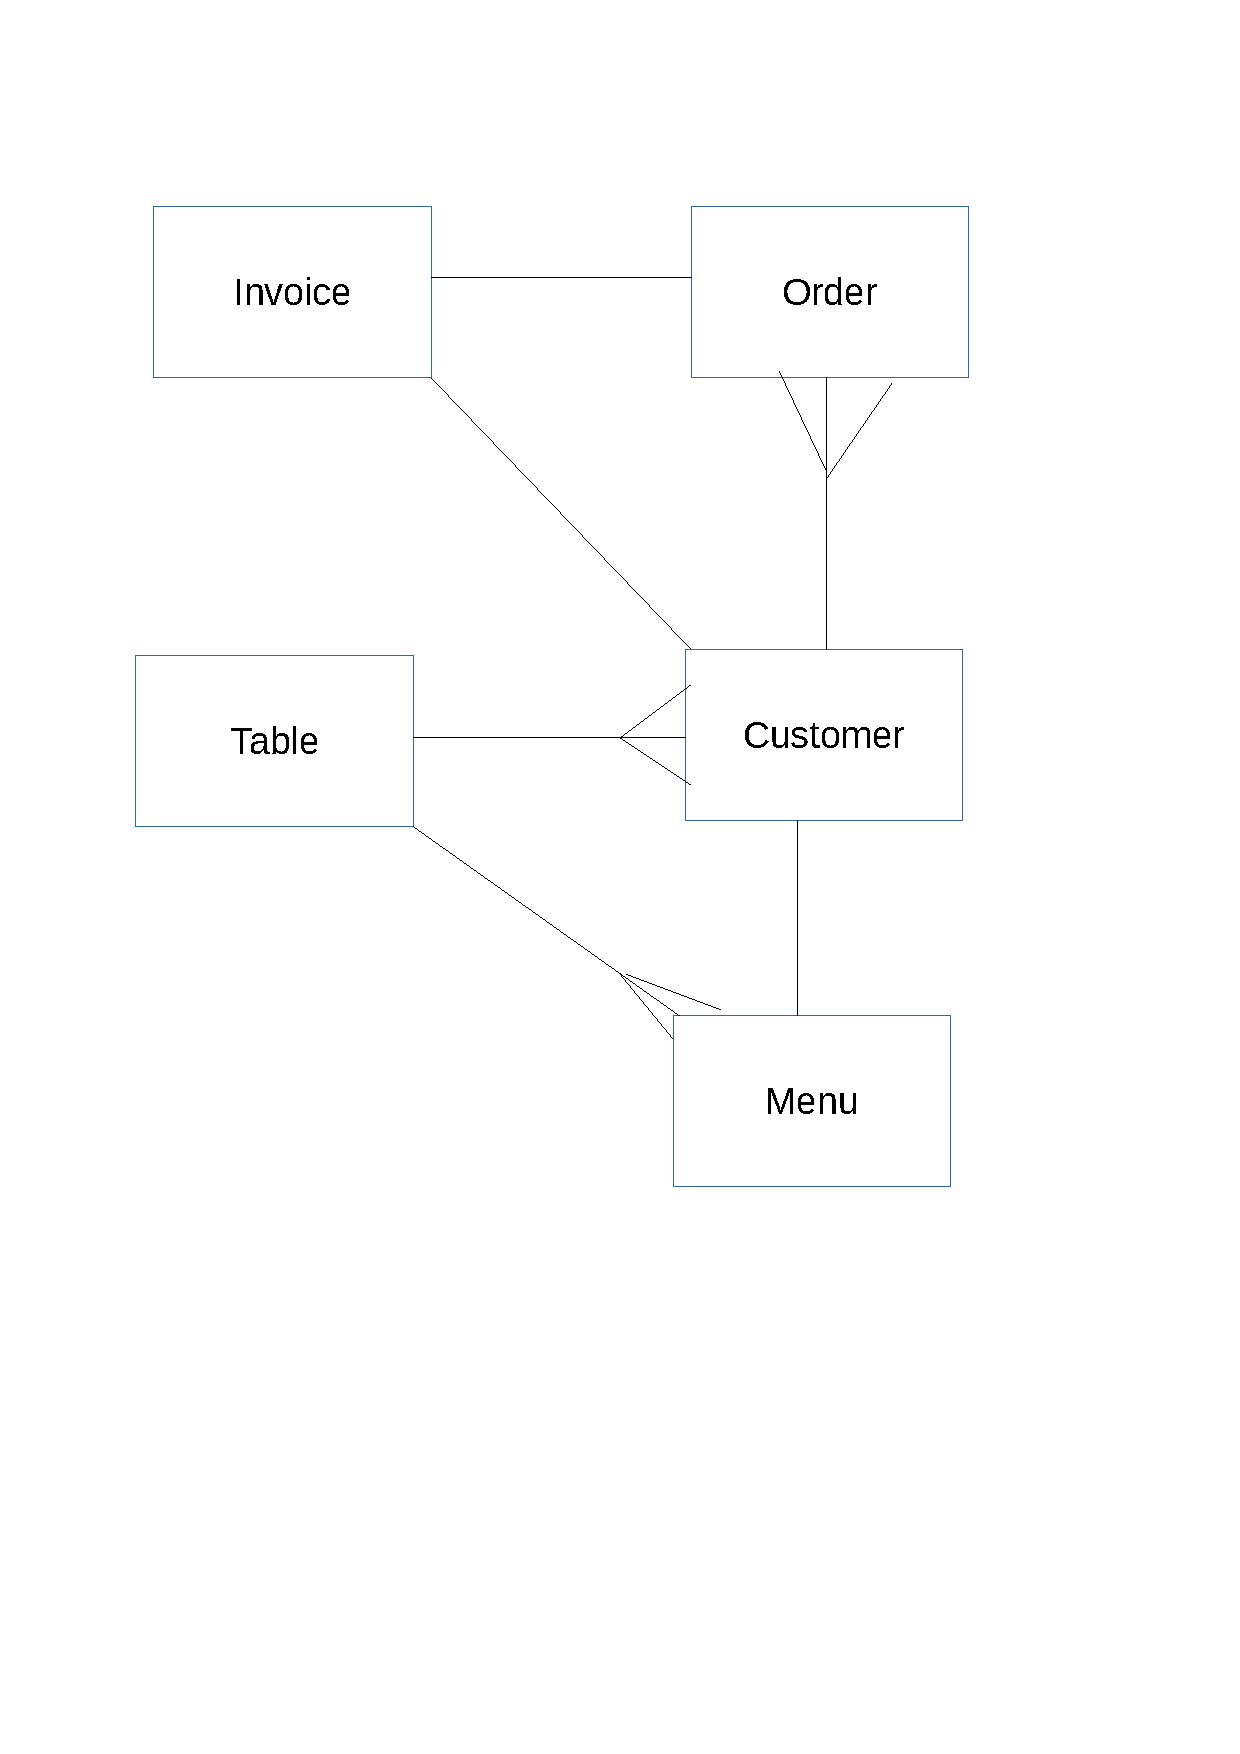
\includegraphics[height = 16cm]{./Analysis/ERDiagram}
    \caption{E-R Diagram} \label{fig:ERD}
\end{figure}

\subsection{Entity Descriptions}

Customer(\underline{CustomerID}, \textit{TableID}, \textit{OrderID}, NumberOfPeople, Invoice, Date)

Order(\underline{OrderID},\textit{CustomerID},\textit{TableID}, \textit{MenuID}, DishOrdered, DrinkOrdered, Quantity)

Table(\underline{TableID}, \textit{OrderID}, \textit{CustomerID}, TableNumber) 

Menu(\underline{MenuID}, Dishes, Drinks, DishPrice, DrinkPrice)

Invoice(\underline{InvoiceID}, \textit{CustomerID}, \textit{OrderID}, TotalDrinkPrice, TotalPrice)


\section{Object Analysis}

\subsection{Object Listing}

\begin {itemize}
	\item Customer
	\item RestaurantStaff
	\item Dish
	\item Drink
	\item Invoice
	\item Menu
\end {itemize}

\subsection{Relationship diagrams}

\begin{figure}[H]
    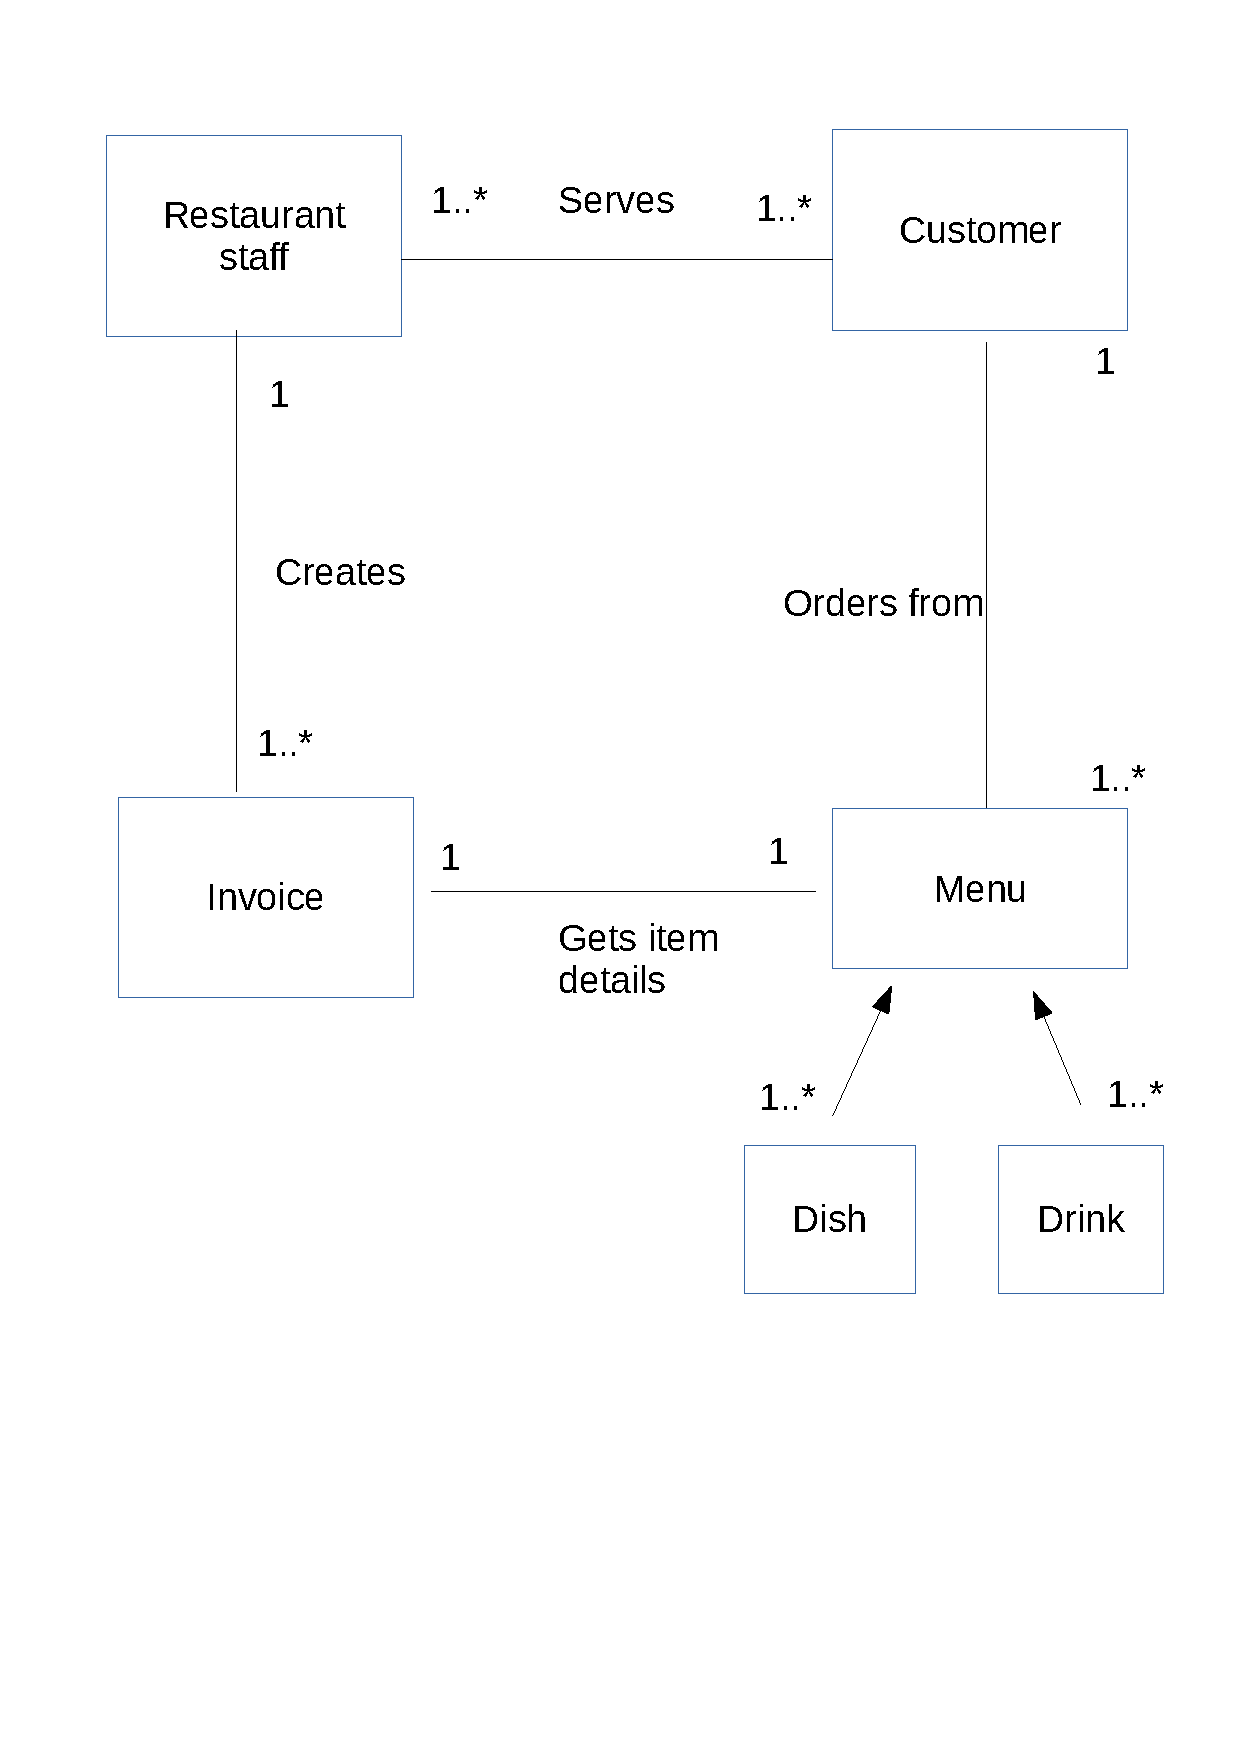
\includegraphics[height = 16cm]{./Analysis/Objects}
    \caption{Relationship diagram} \label{fig:Objects}
\end{figure}

\subsection{Class definitions}

\begin{figure}[H]
    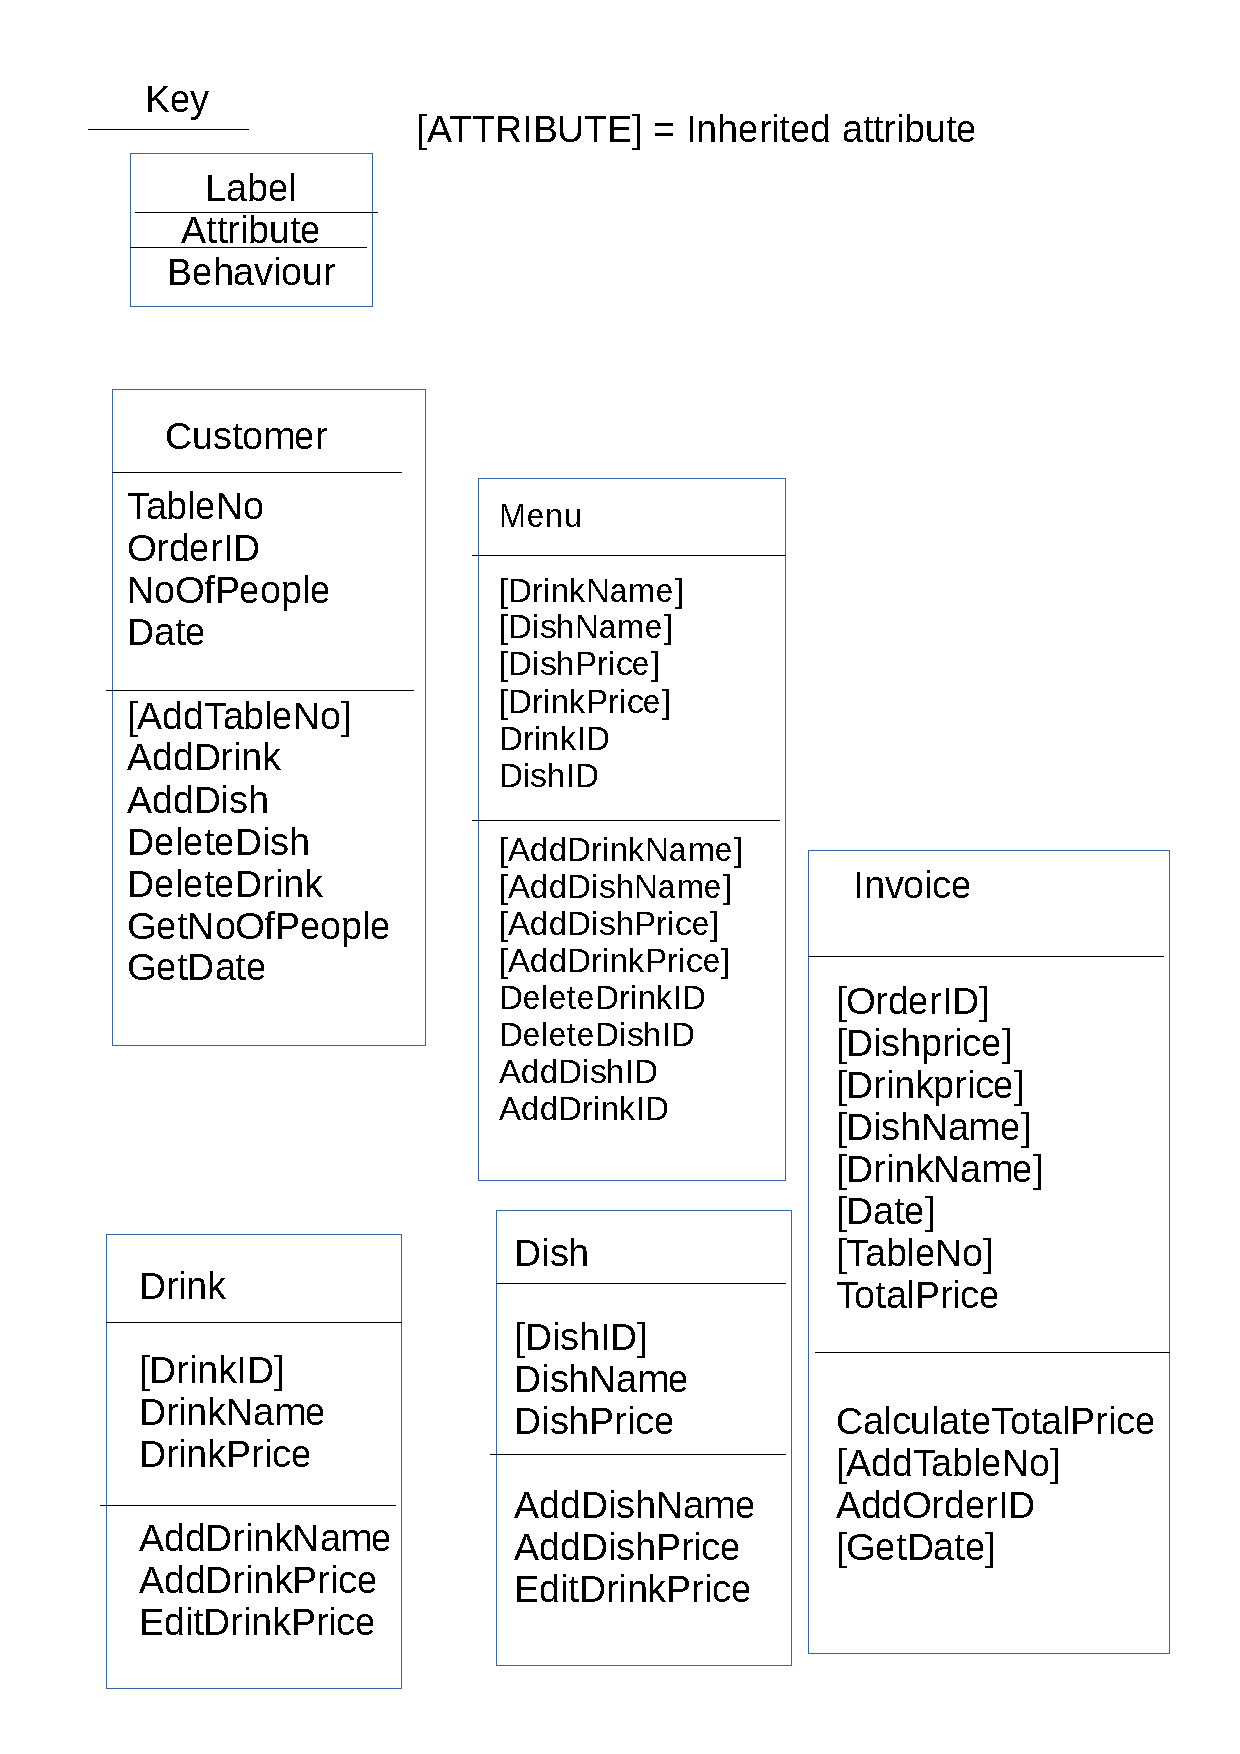
\includegraphics[height = 16cm]{./Analysis/Keyfail}
    \caption{Class diagram} \label{fig:Class}
\end{figure}

\section{Other Abstractions and Graphs}

\section{Constraints}

\subsection{Hardware}
The current computer specifications is as follows:
\begin{itemize}
	\item 19" Display
	\item AMD FX(fm) - 6300 six-core CPU 3.50Hz
	\item 8GB RAM
	\item NViDiA GeForce 9600 GT 1GB
	\item Windows 8.1 64 bit
\end{itemize}

There shouldn't be any constraints apart from the fact that the new system will have to be designed to fit the 19" screen. Also the position of where the computer will be placed in the restaurant is a limitation.

\subsection{Software}

The current computer uses Windows 8.1 and Linh would prefer it to stay that way as she is familiar with the operating system. This is not a problem as the proposed system will run fine on Windows 8.1. Apart from that, Linh has not stated what software can or cannot be used.

\subsection{Time}
Linh has not set me a deadline for the new system and is in no rush for it to get done. Therefore the deadline will be Friday 27th March 2015 which is the coursework deadline set by my teacher.

\subsection{User Knowledge}
Linh has basic knowledge on how to use a computer such as being able to check emails and simple web surfing. Basic knowledge will not constrain the project as one of the objectives is for the software to be simple and clear.


\subsection{Access restrictions}

All working staff should be able to use this software due to the nature on how the business is run. All waiting staff should be able to carry out the same roles such taking an order, serving and creating an invoice form.    However, customers should not be able to access this application at all which could be considered as a constrait. A simple enter password-to-access mechanic could be used as a solution to this.

\section{Limitations}

\subsection{Areas which will not be included in computerisation}

The method of taking orders will not be computerised as it more convenient to just take orders by pad. Using an ordering pad is useful as it is small, light and easy to carry around. Also, the payment system ( receiving money and giving back change) will not be computerised as there are no problems with the current payment system. More problems will likely be created if it was to be computerised such as giving back the correct amount of change and registering the amount of money received.

\subsection{Areas considered for future computerisation}

Tracking bookings for tables can be a feature for later as it could be helpful if the book of table bookings goes missing or if theres no more space to write down bookings. In addition, Linh has not stated that she wanted take aways to be computerised. This could be an additional feature in the future to the program where it creates invoices for take aways.

\section{Solutions}

\subsection{Alternative solutions}

\begin{center}

\begin{tabular}{ | p{2cm} | p{4cm} | p{5cm} |   }
    \hline
    \textbf{Solution} & \textbf{Advantages} & \textbf{Disadvantages} \\ \hline
   Python Desktop Application with a GUI & The design can be changed according to client needs. Not complicated to use. Very low cost. User-friendly and problems with current system will be fixed. Extra features can be implemented. &Application will take up noticeable computer storage. Will take a long 	time to create GUI application. If theres a power cut then system will not be useable \\ \hline
	Touch sceen self-order system & Customer has more freedom.  Less work for restaurant staff. Problems with current system will be gone. & More hardware and software needed - can be very 			costly. Technical issues will be hard to fix. \\ \hline
	Getting someone to do invoices only & Will solve the main problem with current system. No need for a computer. & Will be hard to find someone who will only do invoices. If business isn't busy then invoice person will be almost useless. Could be more costly in long run. \\ \hline
	Redesign current manual system & No cost or very low cost as no computer/software will be needed. Current manual system is simple.& May not be able to fix problems. Will take some time to figure out how to fix problem. \\ \hline


\end{tabular}
\label{tab:Solution_table}
\end{center}


\subsection{Justification of chosen solution}

I have chosen Python Desktop  Application with a GUI  as the solution because of many reasons. One reason is that the touch screen solution will be very costly and customers would have to queue up to use the machine if it gets busy. This will affect how the business will run as many customers do not like to wait. Also, hiring out someone to do invoices will not be efficient as money will be wasted if business is not busy. Furthermore redesigning the current system will take time as Linh would need to figure how fix the problems in the system and also this will most likely not fix most problems with the current system. Therefore I choice Python Desktop Application because it would not need any further hardware, this will not negatively affect customers experience at the restaurant in any way and due to Python being very flexible, the program can always be changed to Linh's wants.
	
